\documentclass[11pt,a4paper]{article}
\usepackage[margin=1in]{geometry}
\usepackage[T1]{fontenc}
\usepackage[utf8]{inputenc}
\usepackage{lmodern}
\usepackage{hyperref}
\usepackage{enumitem}
\usepackage{xurl}
\usepackage{tikz}
\usepackage{float}
\usetikzlibrary{arrows.meta, positioning, shapes.geometric}
\hypersetup{colorlinks=true,linkcolor=blue,urlcolor=blue}
\newcommand{\codepath}[1]{\path{#1}}
\tikzset{box/.style={rectangle,draw,rounded corners,align=center,inner sep=3pt,minimum width=36mm},line/.style={-Latex}}

\title{Phase-1 Deliverable: Output Schema v1}
\author{SIT Engine Architecture}
\date{\today}

\begin{document}
\maketitle

\section{Technical Description}
Output Schema v1 defines stable machine-readable interfaces for window-level and summary-level SIT artifacts.

\section{Implementation Fulfillment}
Schema contract is in \codepath{Phase-1/schema/v1.py} (\texttt{WINDOWS\_COLUMNS}, \texttt{SUMMARY\_KEYS}, validators). Export enforcement is in \codepath{Phase-1/cli.py} \texttt{cmd\_export}, which now validates and writes \texttt{windows\_v1.csv}, \texttt{summary\_v1.json}, and \texttt{windows\_v1.parquet} when parquet backend is available.

\section{Design \& Architecture}
Engine emits internal run artifacts; export stage acts as schema boundary, validating and materializing versioned outputs for downstream consumers.

\subsection*{Function Flowchart}
\begin{figure}[H]
\centering
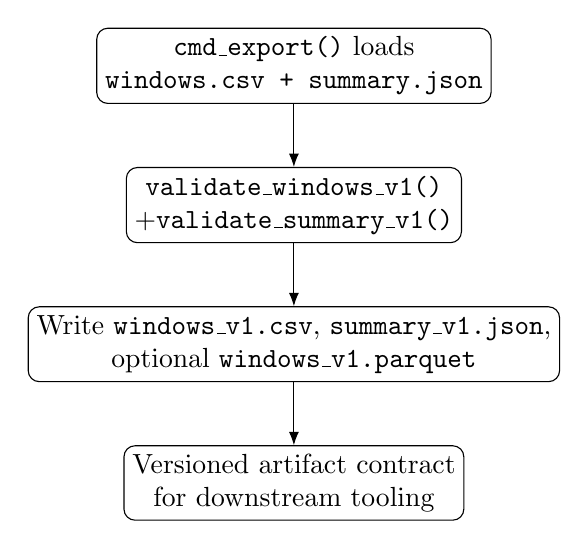
\begin{tikzpicture}[node distance=8mm and 12mm]
\node[box] (a) {\texttt{cmd\_export()} loads\\\texttt{windows.csv + summary.json}};
\node[box, below=of a] (b) {\texttt{validate\_windows\_v1()}\\+\texttt{validate\_summary\_v1()}};
\node[box, below=of b] (c) {Write \texttt{windows\_v1.csv}, \texttt{summary\_v1.json},\\optional \texttt{windows\_v1.parquet}};
\node[box, below=of c] (d) {Versioned artifact contract\\for downstream tooling};
\draw[line] (a) -- (b);
\draw[line] (b) -- (c);
\draw[line] (c) -- (d);
\end{tikzpicture}
\caption{Output Schema v1 Function Flow}
\end{figure}

\end{document}
